\begin{figure}
    \centering
    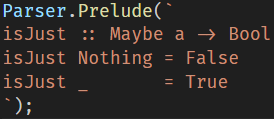
\includegraphics{chapters/6-testing/figures/prelude.png}\\
    \vspace{10mm}
    \begin{tikzpicture}[scale=2,
    type/.style = {
        rectangle, rounded corners,
        draw=black, fill=red!40, drop shadow,
        text centered, anchor=north, text=white, text width=2.6cm,
    },
    thunk/.style = {
        type, fill=blue!40,
    },
    arg/.style = {
        type, fill=purple!40,
    },
    arrow/.style = {
        shorten >= 0.33cm, shorten <= 0.33cm
    }]

    \node (root) [thunk, text width = 3cm] at (0, 2) {FunctionThunk\\isJust};
    
    \node (noth) [arg, text width = 4cm] at (-1.35, 1.1) {ConstructorArgument\\Nothing};
    \node (wild) [arg, text width = 3.5cm] at (1.2, 1) {WildcardArgument};
    
    \node (false) [thunk, text width = 4cm] at (-1.35, 0) {ConstructorThunk\\False};
    \node (true) [thunk, text width = 3.5cm] at (1.2, 0) {ConstructorThunk\\True};
    
    \node (rootT) [type, text width = 3.3cm] at (0, -1) {FunctionType\\Maybe a $\rightarrow$ Bool};
    \node (appT) [type, text width = 3.1cm] at (-1, -2) {ApplicationType\\Maybe a};
    \node (maybeT) [type] at (-2, -3) {LiteralType\\Maybe};
    \node (aT) [type] at (0, -3) {UnboundType\\a};
    \node (boolT) [type] at (1, -2) {LiteralType\\Bool};
    
    \draw[->, arrow] (root) -- (noth);
    \draw[->, arrow] (noth) -- (false);
    \draw[->, arrow] (root) -- (wild);
    \draw[->, arrow] (wild) -- (true);
    
    \draw[->, arrow] (root) -- (rootT);
    \draw[->, arrow] (rootT) -- (appT);
    \draw[->, arrow] (appT) -- (maybeT);
    \draw[->, arrow] (appT) -- (aT);
    \draw[->, arrow] (rootT) -- (boolT);
    
    \end{tikzpicture}
    \caption{The structure of the \texttt{isJust} function. It has 2 patterns with corresponding implementations, and a type.}
    \label{fig:intergration-testing}
\end{figure}